\documentclass[12pt,a4paper]{article}
\usepackage{setspace}
\usepackage{graphicx}
\begin{document}
	\doublespacing
	\tableofcontents
	\newpage
	\section{Title}
	Smart Mobility Autobot for physically disabled using Artificial Intelligence, Morse Code, Voice and Gesture Recognition
	\subsection{Introduction}
	\paragraph{}
	This project aims at improving the lives of the physically challenged with the help of modern technology. The autobot consist of microcontroller, proximity sensor,robotic arm, line follower, motor driver, voice and gesture recognition module and camera. The voice recognition module detects voice of the disabled and is processed by microprocessor to execute the commands like follow, stop, move forward, backward, right, left etc, and acts accordingly.It also identifies the gesture movements of the disabled and moves accordingly. The line follower directs the autobot to move and perform the tasks as per the disabled's instructions within the house. As the physically challenged face problems in movement of things, autobot helps them in delivering the objects from one place to another. The camera is interfaced with the microprocessor for image processing like tracking the objects, recognition and other future scope processes. The autobot tracks the objects and picks it using the robotic arm and places in another place as desired by the disabled person.It has an added feature of SOS,which can be activated by user in emergency. For deafdumb person, the communication is done is through MORSECODE when the message is interpreted by vibrations as dots and dashes. 
	\newpage
	\subsection{Market Research / Literature Survey}
	\paragraph{}
	As Autobot has great features like its compact, strong, cost effective, flexible, feasible, highly efficient, and has a unique technology of voice and gesture recognition which makes the user to use the product easily. It also has many other features which can fulfil the demands of the physically disabled.
	\begin{itemize}
		
		\item It has an added feature of SOS, where the person is in emergency situation, he can call for help just by a single tap of button and autobot sends the message to helplines. The voice is received as vibrations in MORSE CODE that the deaf blind can interpret. With the deaf blind interface, a person uses a combination of DOTS and DASHES to send their messages.
		\item The similar product may not have all these features and may not be affordable. So, the autobot can fulfil all the demands and can stay in the market as compared to others. So, the Autobot is more preferable in the market than the product which is similar to it.
	\end{itemize}
	\section{Hardware requirements:}
	\begin{enumerate}
		\item Microcontroller
		\item Camera
		\item Arduino uno
		\item Servo motor
		\item Motor driver
		\item Proximity sensor
		\item Robotic arm
		\item GPS module
		\item Vibration module
		\item Touch sensor
		\item LEDs / Buzzer / Push button
		\item Battery		content...
	\end{enumerate}
	\section{Software requirements:}
	\begin{enumerate}
		\item TI Connect / Keil micro vision – To control the MCU
		\item MATLAB (2019) – For image processing
		\item Google maps – For GPS tagging
		\item Microsoft Azure machine learning - For machine learning, cloud computing and controlling the bot based on the results of previous activities
		\item Arduino IDE – Controlling the movement of bot and generation of PWM signals on Arduino Uno board
	\end{enumerate}
	\section{Implementation:}
	\paragraph{}
	Core Technical Innovation here is to bring advance technology at present like Artificial Intelligence, voice and gesture recognition. The Morse code is used for the blind and deaf to transmit and interpret the messages and SOS helps the disabled in emergency to contact the help line by a single tap on the Autobot. Uniqueness of product design is COMPACT DESIGN, flexible to move around and carry things (medium weight) on it. These tasks are performed either by voice, gesture recognition making it more efficient to use with great ease. The bot also consists of MORSE CODE converter and SOS feature. Objective: This bot is basically designed after the problems faced by physically challenged people. The disabled instruct the bot by voice or gesture to perform the task like follow, move left, right, backward and forward. For deaf-blind people it has MORSE CODE converter, where it allows such people to understand, what the other person wants to convey and reply back. SOS is an added feature, when the button on the bot is pressed, it calls the nearest possible emergency service.
	\newpage

	\newpage
	\subsection{Block Diagram of the proposed design:}

	
	\begin{figure}
		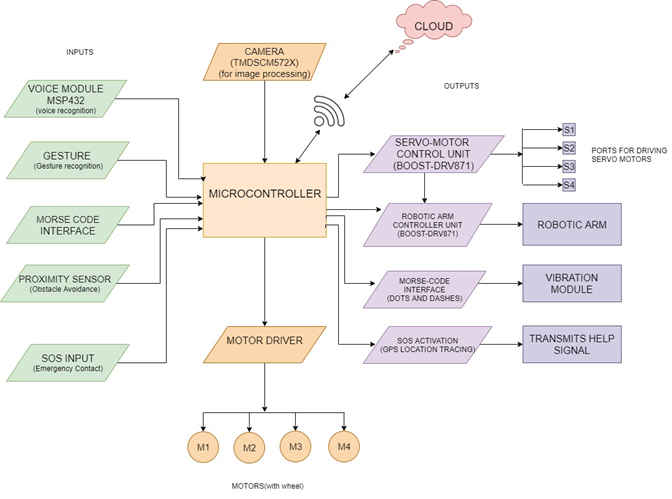
\includegraphics[width=\linewidth]{Blockdiagram.png}
		\caption{Blockdiagram of implementation}
		\label{Figure::blockdiagram}
	\end{figure}

	\subsubsection{Following Processing takes place:}
	\begin{itemize}
		\item[Motor driver]: It is used to drive the autobot from one place to another, which contains four wheels associated with it.
		\item[SOS]: It helps the disabled to contact the helplines in emergency situations by a single tap on the autobot. The autobot sends the message to the nearby helplines with the GPS location of the disabled.
		\item[MORSE CODE]: It is used for the blind and deaf people to communicate through the morse code. Which transmits the signals in the form of dots and dashes. The disabled receive the message through the vibrations.
		\item[Servo Motor control]: (BOOST-DRV871) It is used to drive the servo motor and helps in movement of the robotic arm.
		\item[Robotic arm controller]: It picks and moves the objects from one place to another.
	\end{itemize}
	\paragraph{}
	Microcontroller takes the input from the mentioned input modules and transmits the information to the cloud. Cloud processes the data received and sends back the commands to MCU as to control the peripherals. Microcontroller, then controls the peripherals as per the instructions
	\subsection{Feasibility}
	\paragraph{}
	The problems faced by disabled people is pathetic. Survey shows that there more than 30 million people have difficulty in walking and more than 10 million face ‘vision and hearing’ disability. So, we decided to take latest technology and make the best use of it to help poor disable people  . This project is intended to give disabled people a companion which can help through their daily chores. In order to achieve this, we have put up a camera , robotic arm ,emergency helpline and many other things. These work collectively and acts according to user’s instructions.
	\paragraph{}
	All these activities are completely automated, user does not have to manually describe each instruction all the time just the keyword are said to bot, making it very feasible.
	\newpage
	\section{Reference}
	Ofiicial websites
	\begin{enumerate}
		\item https://azure.microsoft.com/en-in/services/machine-learning/ 
		\item http://www.ti.com/wireless-connectivity/simplelink-solutions/overview/software.html
		\item https://in.mathworks.com/help/matlab/
	\end{enumerate}
	Books
	\begin{enumerate}
		\item Introduction to MATLAB for engineering students by David Houcque, Northwestern University
		content...
	\end{enumerate}
\end{document}
